% Preamble
\documentclass[11pt]{PyRollDocs}

\addbibresource{refs.bib}

% Document
\begin{document}

    \title{The Profile Bulging PyRolL Plugin}
    \author{Christoph Renzing}
    \date{\today}

    \maketitle

    This plugin predicts the free-surface ("bulge" / rounding) shape of a profile's
    cross-section after a rolling pass, i.e. the part of the boundary that is not in
    contact with the rolls. It implements analytical models from the literature for
    both two-roll and three-roll passes, with a particular focus on three-roll (Kocks
    mill / flat-roll block) passes, which is the subject of this restructured version
    of the plugin.

    \section{Model scope}\label{sec:model-scope}

    All models implemented here predict the free-surface shape \emph{given} the
    maximum width $B_1$ of the profile after rolling. How $B_1$ itself is predicted
    (spread prediction) is a separate concern, handled by other PyRolL plugins such as
    \texttt{pyroll-wusatowski-spreading}; this plugin only reshapes the free surface of
    the cross-section consistently with a given (already solved) width. This mirrors
    how the source papers themselves separate the two problems: a spread formula
    calibrated against FE data, and a free-surface-profile formula that consumes the
    predicted spread as an input.

    A generic spread formula such as Wusatowski's needs the equivalent height and
    width of the incoming and outgoing profile, which \texttt{pyroll-core} does not
    define for arbitrary (in particular 3-fold symmetric) cross-sections on its own;
    \texttt{pyroll-lendl-equivalent-method} supplies them via Lendl's equivalent
    rectangle method, including a \texttt{ThreeRollPass}-specific formula. Loading it
    together with a spread-prediction plugin lets a \texttt{ThreeRollPass} predict its
    own out-profile width instead of requiring it to be set explicitly, and is
    recommended for realistic use; Section~\ref{sec:validation} demonstrates the full
    chain (Lendl + Wusatowski + this plugin) end to end.

    \section{Three-roll passes}\label{sec:three-roll}

    Three-roll (Kocks) mills roll a workpiece between three rolls arranged \SI{120}{\degree}
    apart about the pass line, closing in on the stock symmetrically. Two variants are
    modeled, following \textcite{min2003} and \textcite{byon2017} respectively:

    \begin{itemize}
        \item \textbf{Flat-roll mills} \parencite{min2003}: the roll surface is flat
        along its axis (no machined groove); a round bar is progressively formed into
        a hexagonal shape over several passes. \texttt{pyroll-core}'s
        \texttt{FlatGroove} used in a \texttt{ThreeRollPass} models this case
        (\texttt{"flat"} classifier).
        \item \textbf{Kocks mills with a curved (grooved) roll surface}
        \parencite{byon2017}: the roll surface carries a shallow, machined groove
        (radius $D_g/2$), producing a rounded ("Koval") caliber. Any non-flat groove
        used in a \texttt{ThreeRollPass} (round, oval, hexagonal, ...) is treated this
        way.
    \end{itemize}

    Both papers distinguish three types of geometry transition, based on the shape of
    the incoming profile and of the current pass:

    \begin{enumerate}
        \item \textbf{round $\to$ curved-hexagonal / Koval} -- the incoming profile is
        round (\texttt{"round"} in its classifiers).
        \item \textbf{curved-hexagonal $\to$ hexagonal / Koval $\to$ Koval} -- neither
        the incoming profile nor the current pass is round.
        \item \textbf{Koval $\to$ round} -- the current pass itself is round (the final
        pass of a Kocks mill schedule). Min et al. do not treat this case, since their
        experiments never return to a round shape.
    \end{enumerate}

    \subsection{Flat-roll mills (Min et al. 2003)}\label{subsec:min}

    For the round $\to$ curved-hexagonal pass, the free surface is modeled as a
    circular arc, whose center of curvature is offset from the profile's center by an
    eccentricity $e$:
    \[
        \frac{e}{B_0} = 2.40 \cdot \frac{F_H}{F_O}, \qquad R_1 = B_1 - e,
    \]
    where $B_0$ is the incoming profile's own radius (half its maximum width), $B_1$
    the radius of the outgoing profile after rolling, $F_O$ the incoming profile's
    cross-sectional area and $F_H$ the part of it that does not fit the new pass's
    usable cross-section (\texttt{roll\_pass.displaced\_cross\_section} in
    \texttt{pyroll-core}), i.e. the area the roll must displace.

    For the curved-hexagonal $\to$ hexagonal and hexagonal $\to$ hexagonal passes, Min
    et al. approximate the free surface as a \emph{straight chord} instead, from a
    point $W_1$ on the roll face (where contact ends) to the corner tip $B_1$. This
    plugin locates $W_1$ as the point where the roll face crosses the circle of radius
    $B_1$ around the profile's center, on each of the two roll faces flanking a given
    corner, and builds the polygon directly from the resulting $W_1, B_1, W_1$ vertex
    triples at each of the three corners; between corners the boundary follows the
    (straight) roll face exactly, requiring no further approximation there. Min et al.
    note this linear approximation slightly under-predicts the true (mildly curved)
    bulging in this case, with less than 2\% error in cross-sectional area.

    \subsection{Kocks mills (Byon et al. 2017)}\label{subsec:byon}

    All three transition types are modeled as a circular arc with radius of curvature
    $R_s$ and center offset $P_c$ from the profile's center:

    \begin{description}
        \item[round $\to$ Koval] $\displaystyle \frac{P_c}{B_0} = 3.133 \cdot
        \frac{F_H}{F_0}$, \quad $R_s = B_1 - P_c$.
        \item[Koval $\to$ Koval] $P_c = 0$, \quad $R_s = B_1$ (a circle through the
        section's own center).
        \item[Koval $\to$ round] $P_c$ and $R_s$ solve the system
        \[
            R_s = \frac{DS}{2} + P_c, \qquad
            (B_1 \sin 60^\circ)^2 + (B_1 \cos 60^\circ + P_c)^2 = R_s^2,
        \]
        where $DS$ is the current pass's own inscribed circle diameter
        (\texttt{roll\_pass.inscribed\_circle\_diameter}), giving the closed form
        \[
            P_c = \frac{(DS/2)^2 - B_1^2}{B_1 - DS}.
        \]
    \end{description}

    \subsection{Implementation}\label{subsec:three-roll-impl}

    The dispatch between these cases (module \texttt{pyroll.profile\_bulging.three\_roll\_pass})
    is driven purely by classifiers already available on the roll pass and its incoming
    profile -- no additional configuration is required:

    \begin{center}
        \begin{tabular}{lll}
            \toprule
            Condition & Flat roll & Curved (Koval) roll \\
            \midrule
            \texttt{"round" in in\_profile.classifiers} & Min circular arc & Byon round $\to$ Koval \\
            \texttt{"round" in roll\_pass.classifiers} & (not treated by Min) & Byon Koval $\to$ round \\
            otherwise & Min linear chord & Byon Koval $\to$ Koval \\
            \bottomrule
        \end{tabular}
    \end{center}

    The resulting eccentricity and radius of curvature are exposed as the hooks
    \texttt{ThreeRollPass.OutProfile.bulge\_eccentricity} and
    \texttt{ThreeRollPass.OutProfile.bulge\_radius} (the latter is \texttt{None} for
    Min's linear-chord passes, which have no single radius of curvature).

    For the circular-arc cases, the free surface is traced directly, angle by angle,
    as whichever is closer to the profile's center: the nearest corner's bulge circle,
    or the roll's own un-bulged contour (full roll contact). This is deliberately
    \emph{not} built via the union of the three, generally overlapping, corner circles
    intersected with the roll contour, since that is prone to a spurious reentrant
    cusp wherever two such shapes cross without being exactly tangent there. Sampling
    the two candidate radii directly instead guarantees a shape with no self-crossings
    and keeps the residual non-smoothness to a minimum, but cannot remove it
    entirely: two neighboring corners' bulge circles are not, in general, tangent to
    each other or to the roll contour at the point where the model hands off between
    them, so a small change in slope at that point is an inherent feature of
    connecting three independently-fitted per-corner arc formulas into one closed
    cross-section - most visible for a heavily-reduced first (round-input) pass, where
    the eccentricity is large relative to the spacing between corners (see the round
    $\to$ Koval case in Fig.~\ref{fig:validation-byon}). The source papers validate
    each corner's own arc against a one sixth-symmetric sector of FE/experimental data
    (Section~\ref{sec:validation}) and do not themselves address the smoothness of the
    reassembled full cross-section.

    \section{Two-roll passes}\label{sec:two-roll}

    For completeness, and unchanged in this restructuring, the plugin also implements
    the round-oval-round free-surface model of \textcite{lee2000,lee2001,lee2002} and a
    circular-arc construction for square-diamond-square / oval-square passes (module
    \texttt{pyroll.profile\_bulging.two\_roll\_pass}), dispatched analogously by the
    classifiers of the incoming profile and the current pass.

    \section{Validation}\label{sec:validation}

    The three-roll models are validated against the figures of the source papers by
    reproducing their process parameters in PyRolL and comparing the predicted
    cross-section against boundary coordinates digitized from the printed figures. The
    out-profile width is pinned to the digitized shape's own spread tip radius for each
    case (bypassing spread prediction, see Section~\ref{sec:model-scope}), so that only
    the free-surface model itself is being validated. See \texttt{tests/test\_three\_roll\_min\_flat.py},
    \texttt{tests/test\_three\_roll\_byon\_koval.py} and \texttt{tests/test\_three\_roll\_bulge\_formulas.py}
    for the full test code and digitized data (\texttt{tests/data/}); running the test
    suite regenerates the comparison plots under \texttt{tests/output/}.

    \begin{figure}[htbp]
        \centering
        \begin{subfigure}[t]{0.48\textwidth}
            \centering
            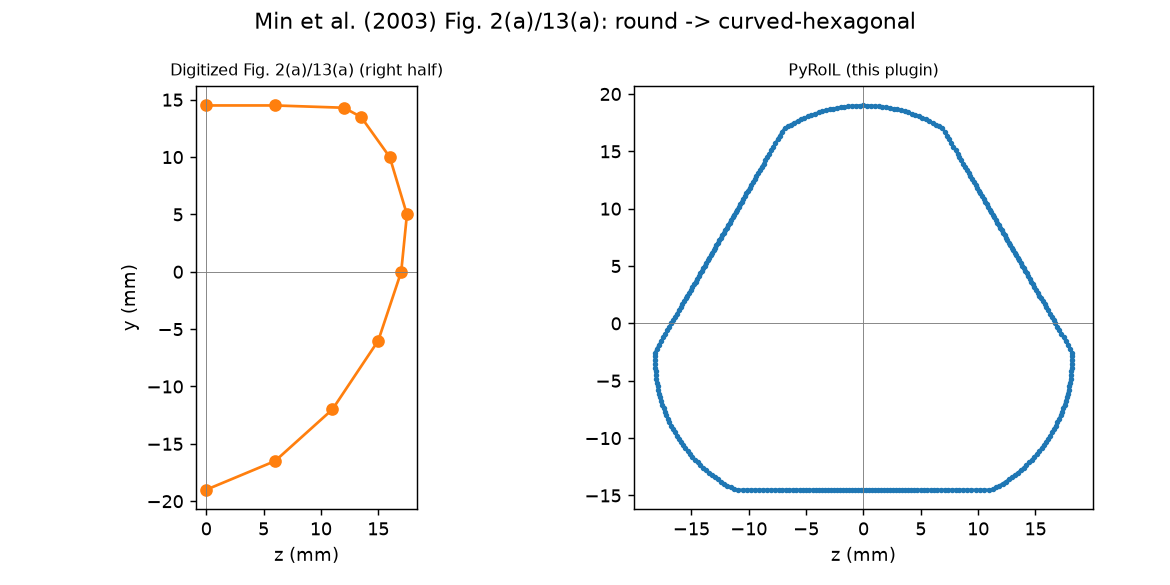
\includegraphics[width=\textwidth]{../tests/output/min_pass_1_round_to_curved_hexagonal.png}
            \caption{Min et al., round $\to$ curved-hexagonal (circular arc).}
        \end{subfigure}
        \hfill
        \begin{subfigure}[t]{0.48\textwidth}
            \centering
            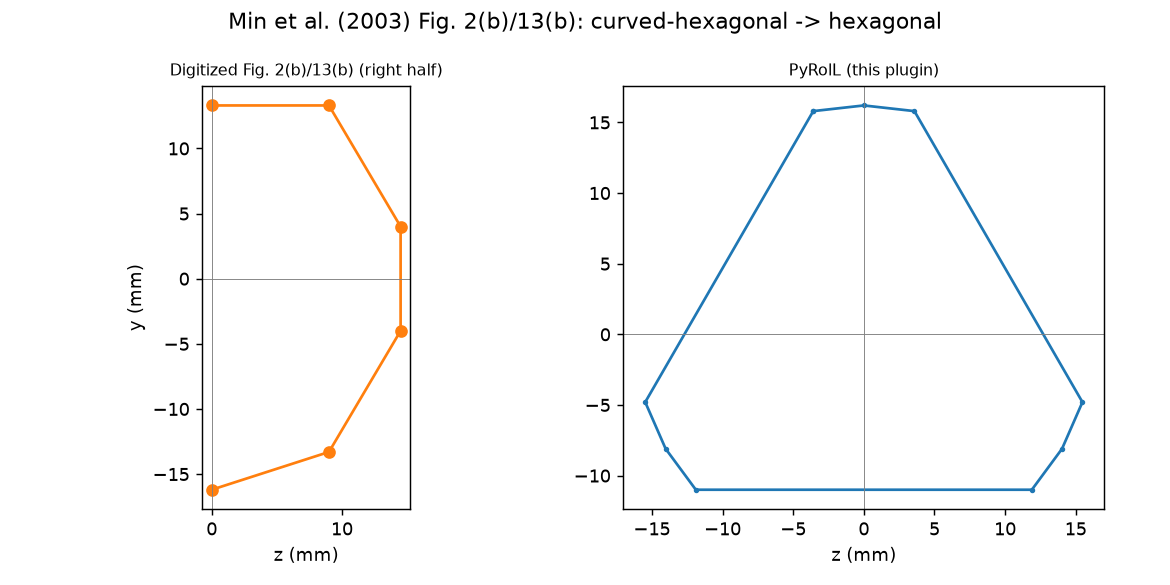
\includegraphics[width=\textwidth]{../tests/output/min_pass_2_curved_hexagonal_to_hexagonal.png}
            \caption{Min et al., curved-hexagonal $\to$ hexagonal (linear chord).}
        \end{subfigure}
        \caption{PyRolL prediction (right) vs. digitized Fig.~2/13 of \textcite{min2003} (left).}
        \label{fig:validation-min}
    \end{figure}

    \begin{figure}[htbp]
        \centering
        \begin{subfigure}[t]{0.48\textwidth}
            \centering
            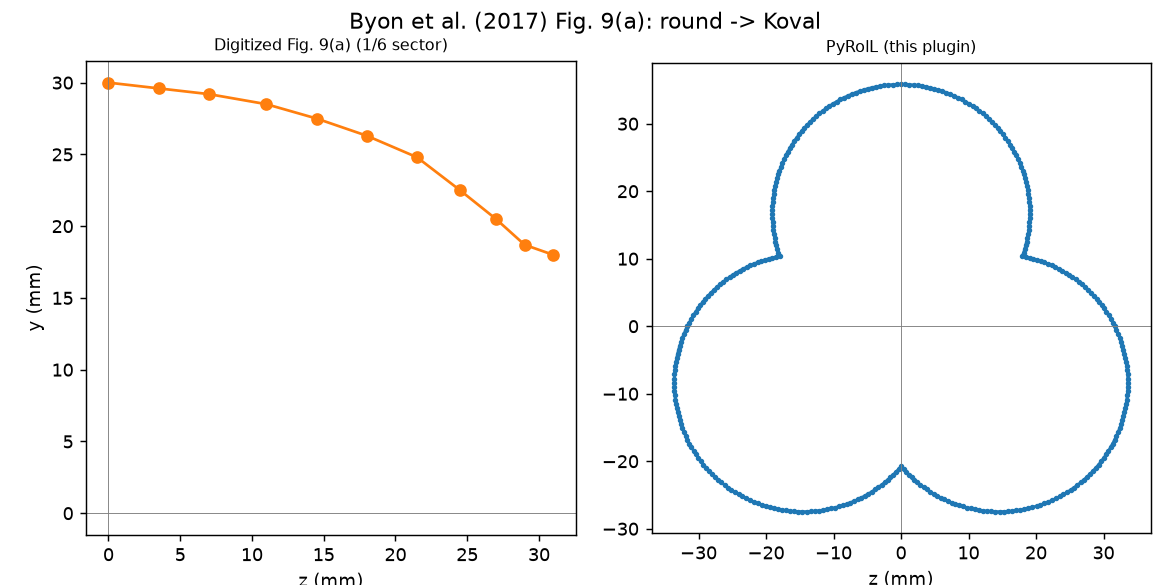
\includegraphics[width=\textwidth]{../tests/output/byon_pass_1_round_to_koval.png}
            \caption{Byon et al., round $\to$ Koval (pass 1).}
        \end{subfigure}
        \hfill
        \begin{subfigure}[t]{0.48\textwidth}
            \centering
            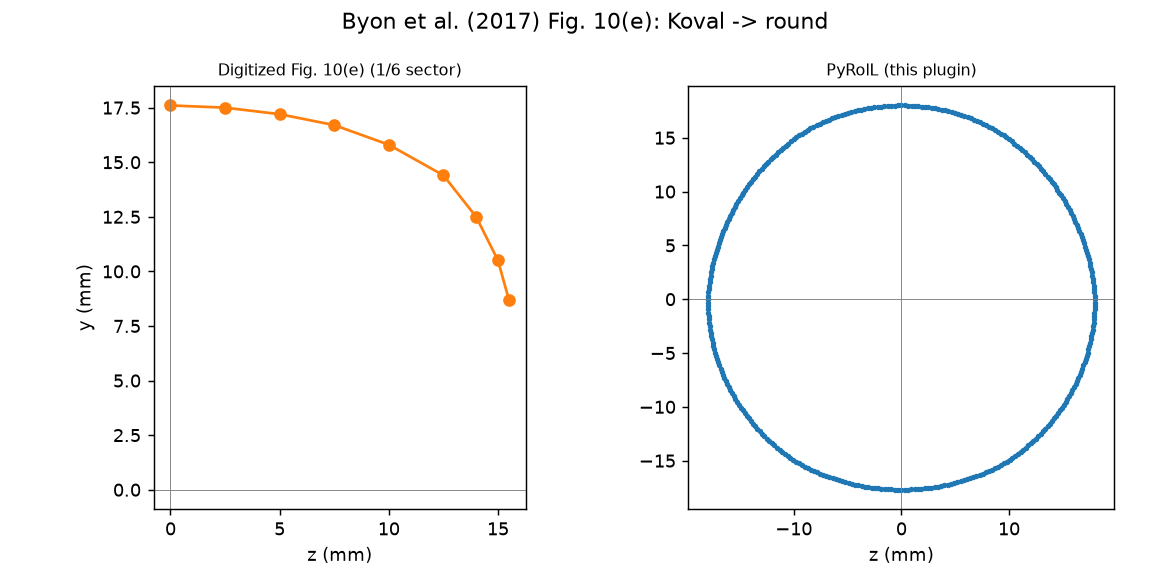
\includegraphics[width=\textwidth]{../tests/output/byon_pass_7_koval_to_round.png}
            \caption{Byon et al., Koval $\to$ round (pass 7, final).}
        \end{subfigure}
        \caption{PyRolL prediction (right) vs. digitized Fig.~9/10 of \textcite{byon2017} (left), 7-pass Kocks mill.}
        \label{fig:validation-byon}
    \end{figure}

    Coordinates were read off 300 dpi page renders of the source PDFs by eye against
    the printed axis gridlines; typical reading uncertainty is $\pm 0.5$--$1$\,mm
    for the millimeter-scale shape plots and $\pm 0.01$--$0.03$ for the dimensionless
    spread/eccentricity calibration plots (Figs.~7, 9, 12). Byon's Figs.~8--10 plot one
    sixth-symmetric sector of the shape in the paper's own local axis orientation,
    which is not necessarily aligned with this plugin's own corner-angle convention;
    those comparisons are therefore shown side by side rather than overlaid.
    \texttt{tests/test\_three\_roll\_bulge\_formulas.py} additionally validates the
    eccentricity coefficients (\num{2.40}, \num{3.133}) directly against the digitized
    FE calibration data of Figs.~7 and 12, and the closed-form Koval $\to$ round
    eccentricity against its defining equations, independent of any PyRolL geometry
    construction.

    \texttt{tests/test\_three\_roll\_end\_to\_end\_spreading.py} complements this with
    a fully predictive (not pinned-width) demonstration: two-pass sequences for both
    mill types, with the out-profile width predicted by
    \texttt{pyroll-wusatowski-\allowbreak spreading} fed by
    \texttt{pyroll-lendl-\allowbreak equivalent-\allowbreak method}
    (Section~\ref{sec:model-scope}), and this plugin's bulging model applying on top
    with no manual intervention, as a real user of the plugin would run it.

    \begin{figure}[htbp]
        \centering
        \begin{subfigure}[t]{0.48\textwidth}
            \centering
            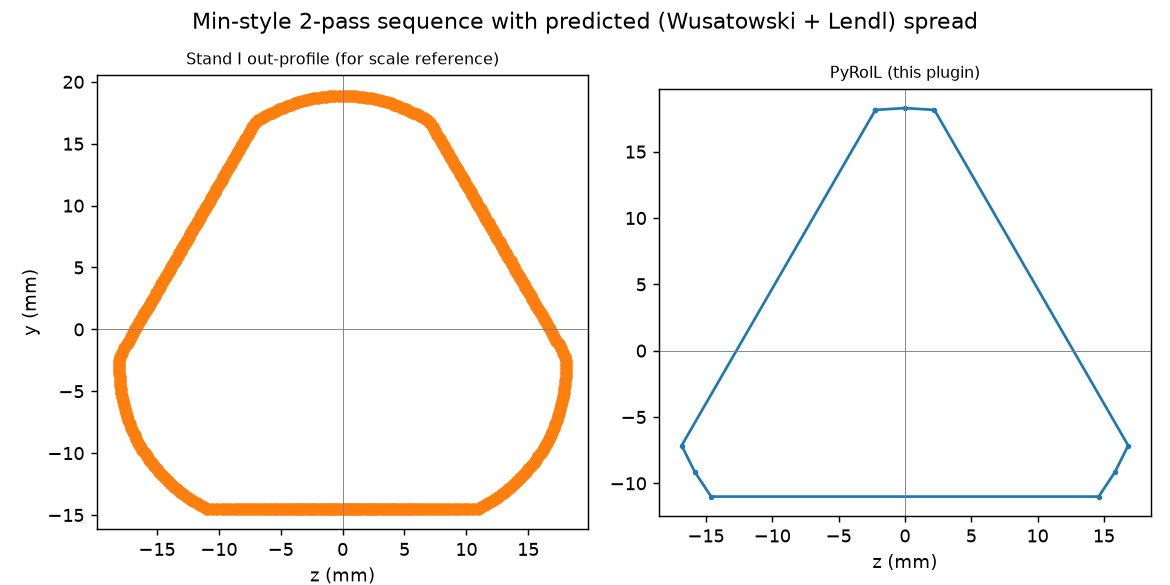
\includegraphics[width=\textwidth]{../tests/output/min_sequence_predicted_spread.png}
            \caption{Min-style flat-roll sequence.}
        \end{subfigure}
        \hfill
        \begin{subfigure}[t]{0.48\textwidth}
            \centering
            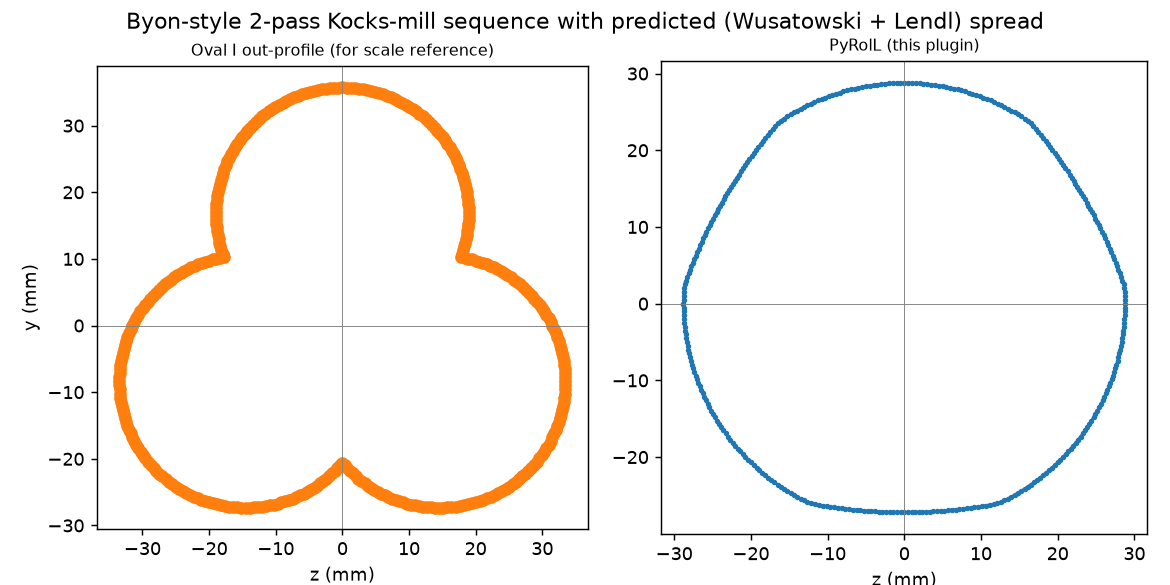
\includegraphics[width=\textwidth]{../tests/output/byon_sequence_predicted_spread.png}
            \caption{Byon-style Kocks-mill sequence.}
        \end{subfigure}
        \caption{Second-pass out-profile (right) with the width predicted end to end by
            Lendl + Wusatowski, shown against the first-pass out-profile for scale
            (left, not a reference shape here).}
        \label{fig:validation-predicted}
    \end{figure}

    \section{Usage instructions}\label{sec:usage-instructions}

    Importing the plugin registers its post-processors on \texttt{TwoRollPass} and
    \texttt{ThreeRollPass}; no further setup is needed. Load a spread-prediction
    plugin and the \texttt{pyroll-lendl-\allowbreak equivalent-\allowbreak method}
    package alongside it (see Section~\ref{sec:model-scope}) to have the out-profile
    width predicted rather than requiring it explicitly:

    %! language = Python
    \begin{minted}{python}
        from pyroll.core import Profile, Roll, ThreeRollPass, FlatGroove
        import pyroll.wusatowski_spreading
        import pyroll.lendl_equivalent_method
        import pyroll.profile_bulging

        in_profile = Profile.round(diameter=35.8e-3, temperature=1323.15, strain=0,
                                    material=["C45", "steel"], flow_stress=100e6,
                                    length=1, density=7.5e3,
                                    specific_heat_capacity=690, thermal_conductivity=23)

        roll_pass = ThreeRollPass(
            roll=Roll(groove=FlatGroove(r1=5e-3, usable_width=45e-3, pad_angle=30),
                      nominal_radius=185e-3, rotational_frequency=248 / 60),
            inscribed_circle_diameter=29e-3,
        )

        out_profile = roll_pass.solve(in_profile)
        print(out_profile.width, out_profile.bulge_radius, out_profile.cross_section.area)
    \end{minted}

    Shell command to build this documentation (requires a working LaTeX installation):

    %! language = Shell Script
    \begin{minted}{shell}
pyroll input.py solve report
    \end{minted}

    \printbibliography

\end{document}
